\documentclass[Chap2main.tex]{subfiles}

% Load any packages needed for this document

\begin{document}
	%-----------------------------------------------------------------------------------%
	%Section 1
	\section{Bland Altman Plots In Literature}
	\citet{mantha} contains a study the use of Bland Altman plots of 44 articles in several named journals over a two year period. 42
	articles used Bland Altman's limits of agreement, wit the other two used correlation and regression analyses. \citet{mantha}
	remarks that 3 papers, from 42 mention predefined maximum width for limits of agreement which would not impair medical care.
	
	The conclusion of \citet{mantha} is that there are several inadequacies and inconsistencies in the reporting of results ,and
	that more standardization in the use of Bland Altman plots is required. The authors recommend the prior determination of limits
	of agreement before the study is carried out. This contention is endorsed by \citet{lin}, which makes a similar recommendation for
	the sample size, noting that\emph{sample sizes required either was not mentioned or no rationale for its choice was given}.
	%-----------------------------------------------------------------------------------%
	%Section 2
	\section{The Bland Altman Plot}
	
	In 1986 Bland and Altman published a paper in the Lancet proposing the difference plot for use for method comparison purposes. It has
	proved highly popular ever since. This is a simple, and widely used , plot of the differences of each data pair, and the
	corresponding average value. An important requirement is that the two measurement methods use the same scale of measurement.
	\\
	Variations of the Bland Altman plot is the use of ratios, in the place of differences.
	\begin{equation}
	D_{i} = X_{i} - Y_{i}   \label{BA01}
	\end{equation}
	Altman and Bland suggest plotting the within subject differences $ D = X_{1} - X_{2} $ on the ordinate versus the average of $x_{1}$
	and  $x_{2}$ on the abscissa. 
	%-----------------------------------------------------------------------------------%
	%Section 3
	\section{Criticism of Bland Altman Plot}
	Unfortunately the Bland-Altman plot has a fatal flaw: it indicates incorrectly that there are systematic differences or bias in the
	relationship between two measures, when one has been calibrated against the other. (Hopkins)
	
	%Section 4
	\section{Bland Altman Plots}
	The issue of whether two measurement methods are comparable to the extent that they can be used interchangeably with sufficient
	accuracy is encountered frequently in scientific research. Historically comparison of two methods of measurement was carried
	out by use of matched pairs correlation coefficients or simple linear regression. Bland and Altman recognized the inadequacies of
	these analyses and articulated quite thoroughly the basis on which of which they are unsuitable for comparing two methods of
	measurement \citep*{BA83}.
	
	As an alternative they proposed a simple statistical methodology specifically appropriate for method comparison studies. They
	acknowledge that there are other valid methodologies, but argue that a simple approach is preferable to complex approaches,
	\emph{``especially when the results must be explained to non-statisticians"} \citep*{BA83}.
	
	The first step recommended, which the authors argue should be mandatory, is construction of a simple scatter plot of the data.
	The line of equality ($X=Y$) should also be shown, as it is necessary to give the correct interpretation of how both methods
	compare. A scatter plot of the Grubbs data is shown in figure 2.1.
	A visual inspection thereof confirms the previous conclusion that there is an inter method bias present, i.e. Fotobalk device has a
	tendency to record a lower velocity.
	
	%\begin{figure}[h!]
	%\begin{center}
	%  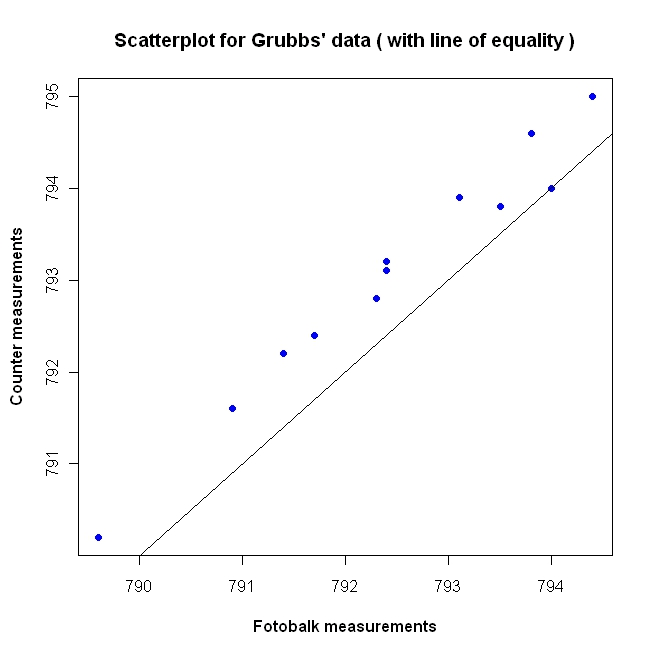
\includegraphics[width=130mm]{GrubbsScatter.jpeg}
	%  \caption{Scatter plot For Fotobalk and Counter Methods}\label{GrubbsScatter}
	%\end{center}
	%\end{figure}
	
	In light of shortcomings associated with scatterplots, \citet*{BA83} recommend a further analysis of the data. Firstly
	differences of measurements of two methods on the same subject should  be calculated, and then the average of those measurements
	(Table 1.1). The averages of the two measurements is considered by Bland and Altman to the best estimate for the unknown true value.
	Importantly both methods must measure with the same units. These  results are then plotted, with differences on the ordinate and
	averages on the abscissa (figure 1.2).
	
	The dashed line in figure 1.2 alludes to the inter method bias between the two methods, as mentioned previously. Bland and Altman
	recommend the estimation of inter method bias by calculating the average of the differences. In the case of Grubbs data the inter
	method bias is $-0.61$ metres per second.
	\newpage
	% latex table generated in R 2.6.0 by xtable 1.5-5 package
	% Thu Aug 27 16:31:52 2009
	\begin{table}[tbh]
		\begin{center}
			
			\begin{tabular}{|c|c|c|c|c|}
				\hline
				Round & Fotobalk [F] & Counter [C] & Differences [F-C] & Averages [(F+C)/2] \\
				\hline
				1 & 793.80 & 794.60 & -0.80 & 794.20 \\
				2 & 793.10 & 793.90 & -0.80 & 793.50 \\
				3 & 792.40 & 793.20 & -0.80 & 792.80 \\
				4 & 794.00 & 794.00 & 0.00 & 794.00 \\
				5 & 791.40 & 792.20 & -0.80 & 791.80 \\
				6 & 792.40 & 793.10 & -0.70 & 792.80 \\
				7 & 791.70 & 792.40 & -0.70 & 792.00 \\
				8 & 792.30 & 792.80 & -0.50 & 792.50 \\
				9 & 789.60 & 790.20 & -0.60 & 789.90 \\
				10 & 794.40 & 795.00 & -0.60 & 794.70 \\
				11 & 790.90 & 791.60 & -0.70 & 791.20 \\
				12 & 793.50 & 793.80 & -0.30 & 793.60 \\
				\hline
			\end{tabular}
			\caption{Fotobalk and Counter Methods: Differences and Averages}
		\end{center}
	\end{table}
	
	%\begin{figure}[h!]
	%\begin{center}
	%  \includegraphics[width=120mm]{GrubbsBAplot.jpeg}
	%  \caption{Bland Altman plot for Fotobalk and Counter methods}\label{GrubbsBA}
	%\end{center}
	%\end{figure}
	\newpage
	
	From a visual inspection of Bland-Altman plot, it is also possible to compare the precision of each method in addition to the
	inter-method bias.  Evidently the data points in the figure 1.2 tend to cluster near the bias line, particularly at the lower end
	of the range of measurements. The variances of the differences seem to increase along the range. In case of small data sets, any
	decision on the level of precision is subjective.
	
	\subsection{Inspecting the Data}
	Bland-Altman plots are a powerful graphical methodology for making a visual assessment of the data. \citet*{BA83} express the
	motivation for this plot thusly:
	\begin{quote}
		"From this type of plot it is much easier to assess the magnitude of disagreement (both error and bias), spot outliers, and see
		whether there is any trend, for example an increase in (difference) for high values. This way of plotting the data is a
		very powerful way of displaying the results of a method comparison study."
	\end{quote}
	
	
	Figures XX YY and ZZ are three Bland-Altman plots derived from simulated data, each for the purpose of demonstrating how the plot
	would inform an analyst of trends that would adversely affect use of the recommended methodology. Figure XX demonstrates how the
	Bland Altman plot would indicate increasing variance of differences over the measurement range.
	
	Figure ZZ is an example of cases where the inter-method bias changes over the measurement range. This is known as proportional
	bias \citep{ludbrook97}.
	
	\newpage
	\begin{figure}[h!]
		\begin{center}
			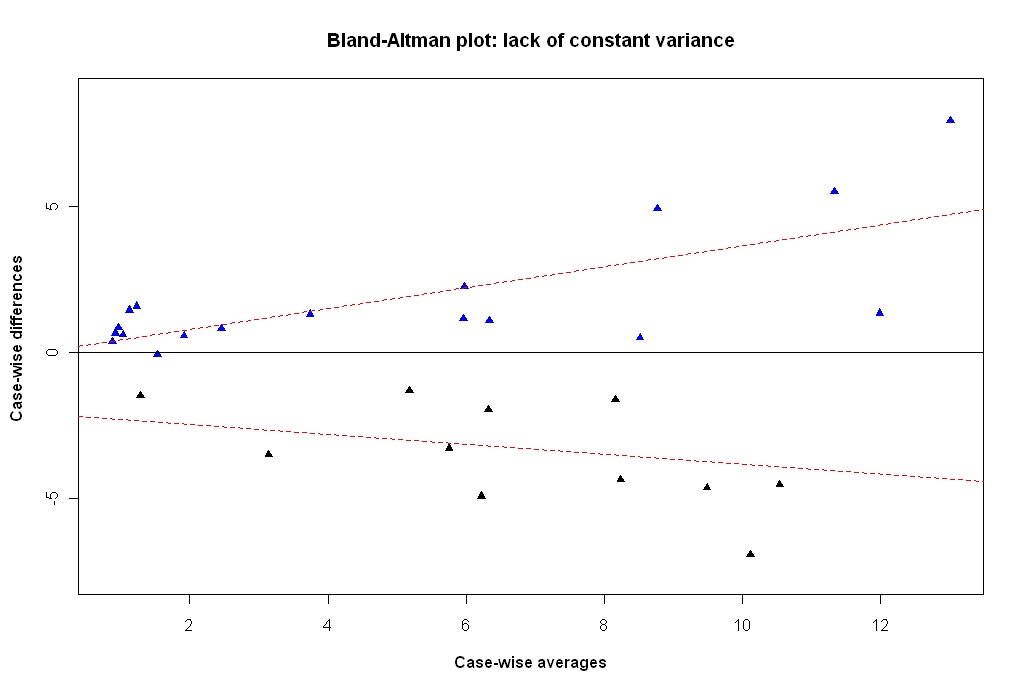
\includegraphics[width=125mm]{BAFanEffect.jpeg}
			\caption{Bland-Altman Plot demonstrating the increase of variance over the range}\label{BAFanEffect}
		\end{center}
	\end{figure}
	
	%\begin{figure}[h!]
	%\begin{center}
	%  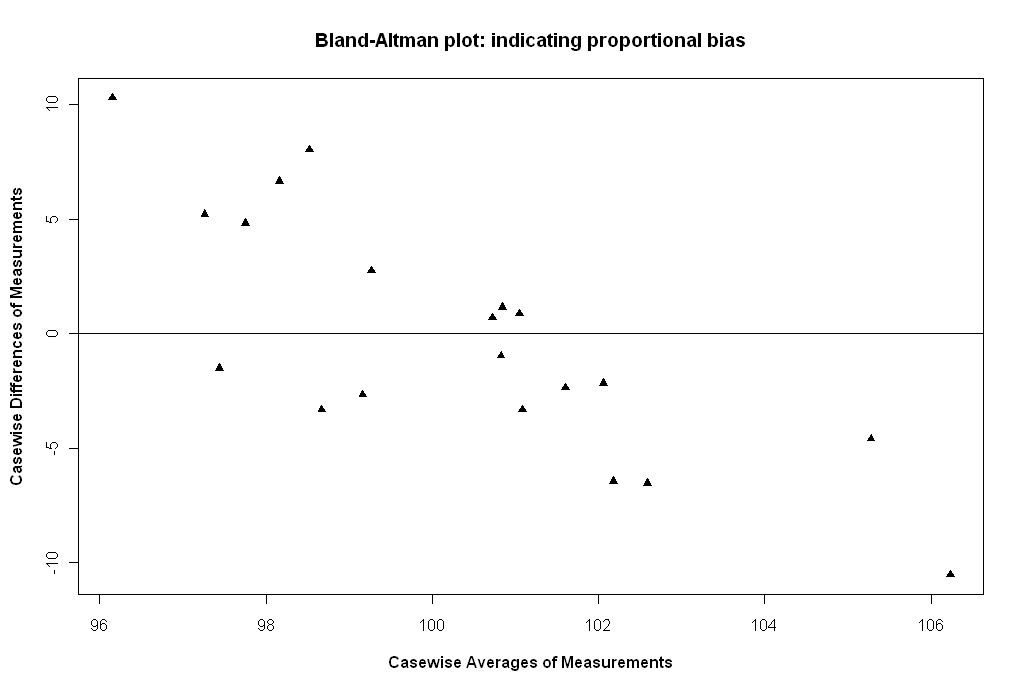
\includegraphics[width=125mm]{PropBias.jpeg}
	%  \caption{Bland-Altman Plot indicating the presence of proportional bias}\label{PropBias}
	%\end{center}
	%\end{figure}
	
	\newpage
	Figure ZZ is an example of cases where the inter-method bias changes over the measurement range. This is known as proportional
	bias (Ludbrook, 1997). Both of these cases violate the assumptions necessary for further analysis using limits of agreement ,which
	shall be discussed later. The plot also can be used to identify outliers. An outlier is an observation that is numerically distant
	from the rest of the data. Classification thereof is a subjective decision in any analysis, but must be informed by the logic of the
	formulation. Figure YY is a Bland Altman plot with two conspicuous observations, at the extreme left and right of the plot
	respectively.
	
	
	\begin{figure}[h!]
		\begin{center}
			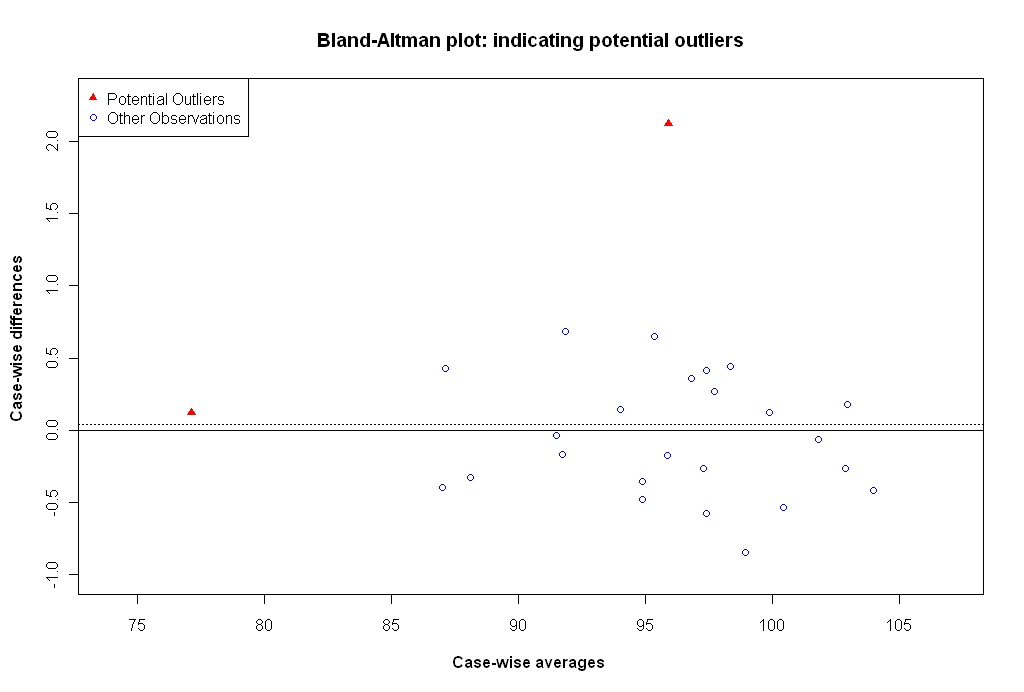
\includegraphics[width=125mm]{BAOutliers.jpeg}
			\caption{Bland-Altman Plot indicating the presence of Outliers}\label{PropBias}
		\end{center}
	\end{figure}
	
	In the Bland-Altman plot, the horizontal displacement of any observation is supported by two independent measurements. Hence
	any observation , such as the one on the extreme right of figure YY, should not be considered an outlier on the basis of a
	noticeable horizontal displacement from the main cluster. The one on the extreme left should be considered an outlier, as it has a
	noticeable vertical displacement from the rest of the observations.
	
	\citet*{BA99} do not recommend excluding outliers from analyses. However recalculation of the inter-method bias estimate , and
	further calculations based upon that estimate, are useful for assessing the influence of outliers.\citep{BA99} states that
	\emph{"We usually find that this method of analysis is not too sensitive to one or two large outlying differences."}
	
	\newpage
	\section{Limits of Agreement}
	\citet{BA86} introduces an elaboration of the plot, adding to the plot `limits of agreement' to the plot. These limits are based
	upon the standard deviation of the differences. The discussion shall be reverted to these limits of agreement in due course.
	
	\subsection{Variations of the Bland Altman Plot}
	\citet{BA99} remarks that it is possible to ignore the issue altogether, but the limits of agreement would wider apart than
	necessary when just lower magnitude measurements are considered. Conversely the limits would be too narrow should only higher
	magnitude measurements be used. To address the issue, they propose the logarithmic transformation of the data. The plot is then
	formulated as the difference of paired log values against their mean. \citet{BA99} acknowledge that this is not easy to interpret,
	and that it is not suitable in all cases.
	
	\citet{BA99} offers two variations of the Bland -Altman plot that are intended to overcome potential problems that the conventional
	plot would inappropriate for.
	
	The first variation is a plot of casewise differences as percentage of averages, and is appropriate when there is an
	increase in variability of the differences as the magnitude increases.
	
	
	% When selecting this option the differences will be expressed as
	% percentage of the averages. This option is useful when there is an
	% increase in variability of the differences as the magnitude of the
	% measurement increases.
	
	\section{Bland Altman Plots}
	The issue of whether two measurement methods are comparable to the extent that they can be used interchangeably with sufficient
	accuracy is encountered frequently in scientific research. Historically comparison of two methods of measurement was carried
	out by use of matched pairs correlation coefficients or simple linear regression. Bland and Altman recognized the inadequacies of
	these analyses and articulated quite thoroughly the basis on which of which they are unsuitable for comparing two methods of
	measurement \citep*{BA83}.
	
	As an alternative they proposed a simple statistical methodology specifically appropriate for method comparison studies. They
	acknowledge that there are other valid methodologies, but argue that a simple approach is preferable to complex approaches,
	\emph{"especially when the results must be explained to non-statisticians"} \citep*{BA83}.
	
	The first step recommended which the authors argue should be mandatory is construction of a simple scatter plot of the data.
	The line of equality ($X=Y$) should also be shown, as it is necessary to give the correct interpretation of how both methods
	compare. A scatter plot of the Grubbs data is shown in figure 2.1. A visual inspection thereof confirms the previous conclusion that
	there is an inter method bias present, i.e. Fotobalk device has a tendency to record a lower velocity.
	
	%\begin{figure}[h!]
	%\begin{center}
	%  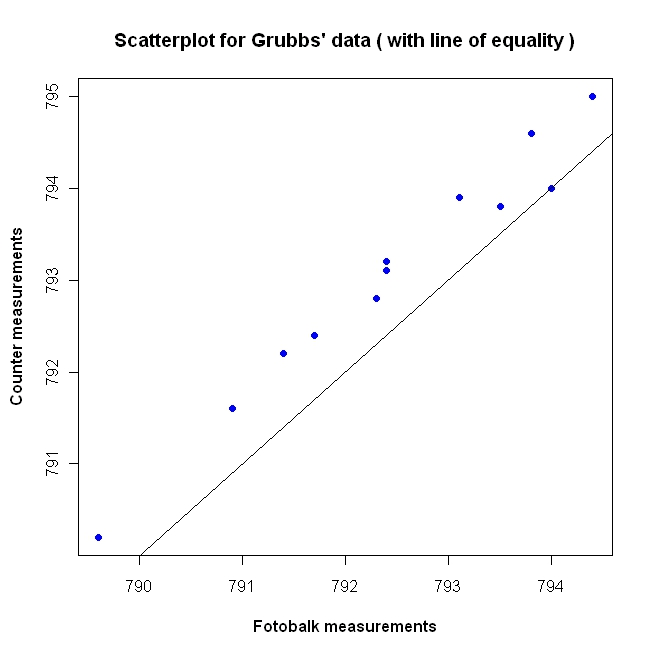
\includegraphics[width=130mm]{GrubbsScatter.jpeg}
	%  \caption{Scatter plot For Fotobalk and Counter Methods}\label{GrubbsScatter}
	%\end{center}
	%\end{figure}
	
	In light of shortcomings associated with scatterplots,
	\citet*{BA83} recommend a further analysis of the data. Firstly differences of measurements of two methods on the same subject
	should  be calculated, and then the average of those measurements (Table 1.1). The averages of the two measurements is considered by
	Bland and Altman to the best estimate for the unknown true value. Importantly both methods must measure with the same units. These
	results are then plotted, with differences on the ordinate and averages on the abscissa (figure 1.2). \citet*{BA83}express the
	motivation for this plot thusly:
	\begin{quote}
		"From this type of plot it is much easier to assess the magnitude of disagreement (both error and bias), spot outliers, and see
		whether there is any trend, for example an increase in (difference) for high values. This way of plotting the data is a
		very powerful way of displaying the results of a method comparison
		study."
	\end{quote}
	\newpage
	% latex table generated in R 2.6.0 by xtable 1.5-5 package
	% Thu Aug 27 16:31:52 2009
	\begin{table}[tbh]
		\begin{center}
			
			\begin{tabular}{|c|c|c|c|c|}
				\hline
				Round & Fotobalk [F] & Counter [C] & Differences [F-C] & Averages [(F+C)/2] \\
				\hline
				1 & 793.80 & 794.60 & -0.80 & 794.20 \\
				2 & 793.10 & 793.90 & -0.80 & 793.50 \\
				3 & 792.40 & 793.20 & -0.80 & 792.80 \\
				4 & 794.00 & 794.00 & 0.00 & 794.00 \\
				5 & 791.40 & 792.20 & -0.80 & 791.80 \\
				6 & 792.40 & 793.10 & -0.70 & 792.80 \\
				7 & 791.70 & 792.40 & -0.70 & 792.00 \\
				8 & 792.30 & 792.80 & -0.50 & 792.50 \\
				9 & 789.60 & 790.20 & -0.60 & 789.90 \\
				10 & 794.40 & 795.00 & -0.60 & 794.70 \\
				11 & 790.90 & 791.60 & -0.70 & 791.20 \\
				12 & 793.50 & 793.80 & -0.30 & 793.60 \\
				\hline
			\end{tabular}
			\caption{Fotobalk and Counter Methods: Differences and Averages}
		\end{center}
	\end{table}
	
	The dashed line in figure 1.2 alludes to the inter method bias
	between the two methods, as mentioned previously. Bland and Altman
	recommend the estimation of inter method bias by calculating the
	average of the differences. In the case of Grubbs data the inter
	method bias is $-0.61$ metres per second.
	\newpage
	%\begin{figure}[h!]
	%\begin{center}
	%  \includegraphics[width=120mm]{GrubbsBAplot.jpeg}
	%  \caption{Bland Altman plot for Fotobalk and Counter methods}\label{GrubbsBA}
	%\end{center}
	%\end{figure}
	
	From a visual inspection of Bland-Altman plot, it is also possible
	to compare the precision of each method in addition to the
	inter-method bias.  Evidently the data points in the figure HH
	tend to cluster near the bias line, particularly at the lower end
	of the range of measurements. The variances of the differences
	seem to increase along the range. In case of small data sets, Any
	decision on the level of precision is subjective.
	
	Figures XX and ZZ are Bland-Altman plots of data simulated for
	expository purposes. Figure XX demonstrates how the Bland Altman
	plot would indicate increasing variance of differences over the
	measurement range. Figure ZZ is an example of cases where the
	inter-method bias changes over the measurement range. This is
	known as proportional bias \citep{ludbrook97}.
	
	\newpage
	\begin{figure}[h!]
		\begin{center}
			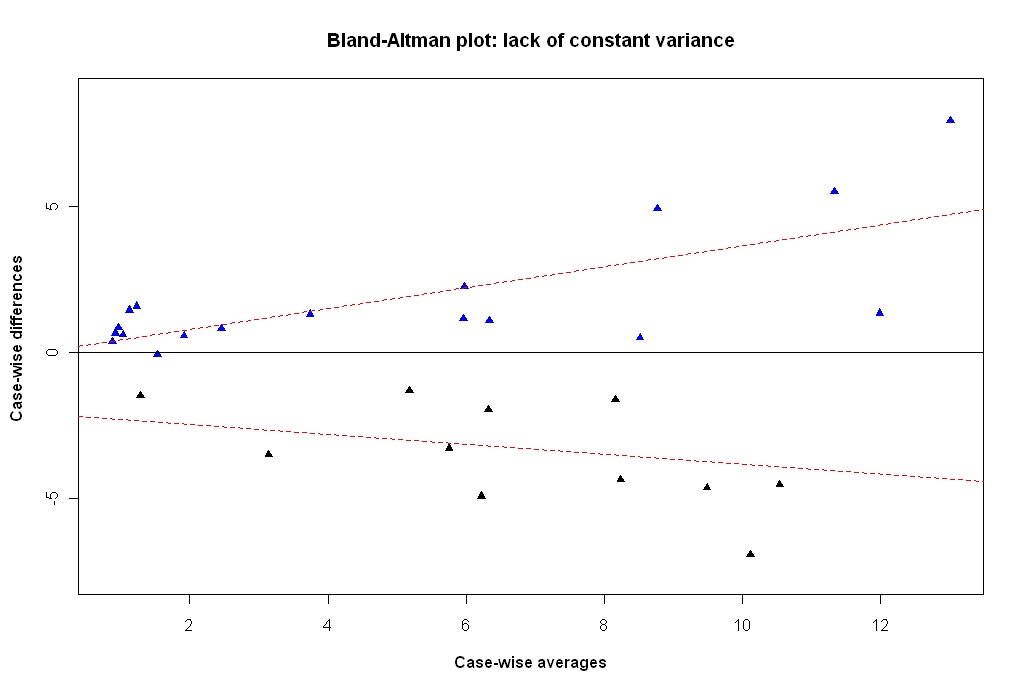
\includegraphics[width=125mm]{BAFanEffect.jpeg}
			\caption{Bland-Altman Plot demonstrating the increase of variance over the range}\label{BAFanEffect}
		\end{center}
	\end{figure}
	%\begin{figure}[h!]
	%\begin{center}
	%  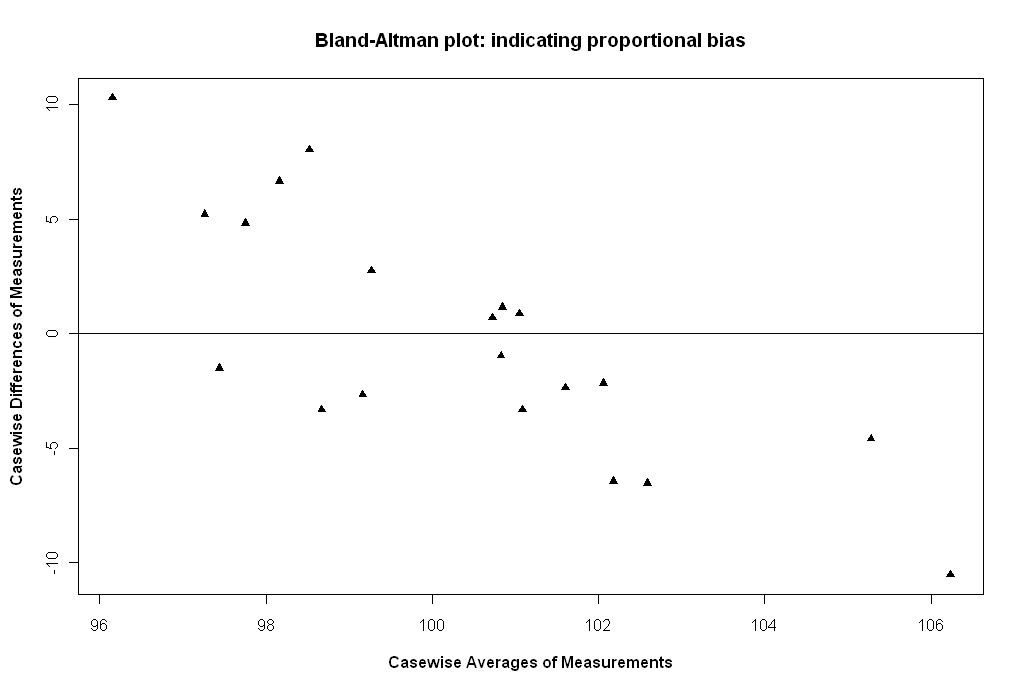
\includegraphics[width=125mm]{PropBias.jpeg}
	%  \caption{Bland-Altman Plot indicating the presence of proportional bias}\label{PropBias}
	%\end{center}
	%\end{figure}
	\newpage
	
	
	
	The fourth pair of measurements from table 1.1 show both methods
	recording the same value, hence the difference is zero. In
	assessing the impact of the corresponding data point, two
	conflicting conclusions can be drawn.
	
	One conclusion is that it is an outlier, and the precision of the
	differences is consistent along the range of measurements. The
	other conclusion is that is not an outlier, and the precision
	increases proportionately along the range of measurements.
	
	The Bland Altman plot is a simple tool for inspection of the data,
	but in itself it offers no formal testing procedure in this
	regard. To this end, the approach proposed by \citet{BA83} is a
	formal test on the Pearson correlation coefficient  of casewise
	differences and means ($\rho_{AD}$). According to the authors,
	this test is equivalent to a well established tests for equality
	of variances, known as the `Pitman Morgan Test' \citep{Pitman,
		Morgan}.
	
	For the Grubbs data, the correlation coefficient estimate
	($r_{AD}$) is 0.2625, with a 95\% confidence interval of (-0.366,
	0.726) estimated by Fishers 'r to z' transformation \citep{Cohen}.
	The null hypothesis ($\rho_{AD}$ =0) would fail to be rejected.
	Consequently the null hypothesis of equal variances of each method
	would also fail to be rejected.
	
	There has no been no further mention of this particular test in
	the subsequent article published by Bland and Altman, although
	\citet{BA99} refers to Spearmans' rank correlation coefficient.
	
	The second variation is a plot of casewise ratios as percentage of
	averages.
	
	% Plot ratios When this option is selected then the ratios of the
	% measurements will be plotted instead of the differences (avoiding
	% the need for log transformation). This option as well is useful
	% when there is an increase in variability of the differences as the
	% magnitude of the measurement increases.
	
	
	\section{Bland Altman plot and the Treatment of Outliers}
	We wish to determine how outliers should be treated in a Bland
	Altman Plot.In their 1983 paper Bland and Altman  merely state
	that the plot can be used to 'spot outliers'. However they pay
	more attention to the issue of outliers in their $1986$ paper,
	wherein they present a data set with an extreme outlier.
	
	
	
	
	In light of shortcomings associated with scatterplots,
	\citet*{BA83} recommend a further analysis of the data. Firstly
	differences of measurements of two methods on the same subject
	should  be calculated, and then the average of those measurements
	(Table 1.1). The averages of the two measurements is considered by
	Bland and Altman to the best estimate for the unknown true value.
	Importantly both methods must measure with the same units. These
	results are then plotted, with differences on the ordinate and
	averages on the abscissa (figure 1.2). \citet*{BA83}express the
	motivation for this plot thusly:
	\begin{quote}
		"From this type of plot it is much easier to assess the magnitude
		of disagreement (both error and bias), spot outliers, and see
		whether there is any trend, for example an increase in
		(difference) for high values. This way of plotting the data is a
		very powerful way of displaying the results of a method comparison
		study."
	\end{quote}
	\newpage
	% latex table generated in R 2.6.0 by xtable 1.5-5 package
	% Thu Aug 27 16:31:52 2009
	\begin{table}[tbh]
		\begin{center}
			
			\begin{tabular}{|c|c|c|c|c|}
				\hline
				Round & Fotobalk [F] & Counter [C] & Differences [F-C] & Averages [(F+C)/2] \\
				\hline
				1 & 793.80 & 794.60 & -0.80 & 794.20 \\
				2 & 793.10 & 793.90 & -0.80 & 793.50 \\
				3 & 792.40 & 793.20 & -0.80 & 792.80 \\
				4 & 794.00 & 794.00 & 0.00 & 794.00 \\
				5 & 791.40 & 792.20 & -0.80 & 791.80 \\
				6 & 792.40 & 793.10 & -0.70 & 792.80 \\
				7 & 791.70 & 792.40 & -0.70 & 792.00 \\
				8 & 792.30 & 792.80 & -0.50 & 792.50 \\
				9 & 789.60 & 790.20 & -0.60 & 789.90 \\
				10 & 794.40 & 795.00 & -0.60 & 794.70 \\
				11 & 790.90 & 791.60 & -0.70 & 791.20 \\
				12 & 793.50 & 793.80 & -0.30 & 793.60 \\
				\hline
			\end{tabular}
			\caption{Fotobalk and Counter Methods: Differences and Averages}
		\end{center}
	\end{table}
	
	The dashed line in figure 1.2 alludes to the inter method bias
	between the two methods, as mentioned previously. Bland and Altman
	recommend the estimation of inter method bias by calculating the
	average of the differences. In the case of Grubbs data the inter
	method bias is $-0.61$ metres per second.
	
	
	From a visual inspection of Bland-Altman plot, it is also possible
	to compare the precision of each method in addition to the
	inter-method bias.  Evidently the data points in the figure HH
	tend to cluster near the bias line, particularly at the lower end
	of the range of measurements. The variances of the differences
	seem to increase along the range. In case of small data sets, Any
	decision on the level of precision is subjective.
	
	Figures XX and ZZ are Bland-Altman plots of data simulated for
	expository purposes. Figure XX demonstrates how the Bland Altman
	plot would indicate increasing variance of differences over the
	measurement range. Figure ZZ is an example of cases where the
	inter-method bias changes over the measurement range. This is
	known as proportional bias \citep{ludbrook97}.
	
	
	
	
	The fourth pair of measurements from table 1.1 show both methods
	recording the same value, hence the difference is zero. In
	assessing the impact of the corresponding data point, two
	conflicting conclusions can be drawn.
	
	One conclusion is that it is an outlier, and the precision of the
	differences is consistent along the range of measurements. The
	other conclusion is that is not an outlier, and the precision
	increases proportionately along the range of measurements.
	
	The Bland Altman plot is a simple tool for inspection of the data,
	but in itself it offers no formal testing procedure in this
	regard. To this end, the approach proposed by \citet{BA83} is a
	formal test on the Pearson correlation coefficient  of casewise
	differences and means ($\rho_{AD}$). According to the authors,
	this test is equivalent to a well established tests for equality
	of variances, known as the `Pitman Morgan Test' \citep{Pitman,
		Morgan}.
	
	For the Grubbs data, the correlation coefficient estimate
	($r_{AD}$) is 0.2625, with a 95\% confidence interval of (-0.366,
	0.726) estimated by Fishers 'r to z' transformation \citep{Cohen}.
	The null hypothesis ($\rho_{AD}$ =0) would fail to be rejected.
	Consequently the null hypothesis of equal variances of each method
	would also fail to be rejected.
	
	There has no been no further mention of this particular test in
	the subsequent article published by Bland and Altman, although
	\citet{BA99} refers to Spearmans' rank correlation coefficient.
	
	\subsection{Criticism of Bland Altman Plot}
	Hopkins[$8$] argues that the plot indicates incorrectly that there
	are systematic differences or bias in the relationship between two
	measures, when one has been calibrated against the other.
	\\
	An Evaluation of the correlation between the difference and means
	complement the analysis.
	\\
	Bland and Altman caution that the calculations are based on the
	assumption that the data is normally distributed. This can be
	verified by using a histogram. If Data is not normally
	distributed, it can be transformed.
	\newpage
	\subsection{Treatment of Outliers}
	Bland and Altman attend to the issue of outliers in their 1986 paper, wherein they present a data set with an extreme outlier
	%-----------------------------------------------------------------------------------%
	\section{Bland Altman plot and the Treatment of Outliers}
	We wish to determine how outliers should be treated in a Bland
	Altman Plot.In their 1983 paper Bland and Altman  merely state
	that the plot can be used to 'spot outliers'. However they pay
	more attention to the issue of outliers in their $1986$ paper,
	wherein they present a data set with an extreme outlier.
	\\
	In Bland and Altman's 1999 paper, we get the clearest indication
	of what Bland and Altman suggest on how to react to the presence
	of outliers. Their recommendation is to recalculate the limits
	without them, in order to test the difference with the calculation
	where outliers are retained. \emph{The span has reduced from 77 to
		59 mmHg, a noticeable but not particularly large reduction.}
	However, they do not recommend removing outliers. Furthermore,
	they say: \emph{We usually find that this method of analysis is
		not too sensitive to one or two large outlying differences.}
	\\
	\\
	In  their $1986$ paper, Bland and Altman give an example of an
	outlier. They state that it could be omitted in practice, but make
	no further comments on the matter.
	\\
	We ask if this would be so in all cases. Given that the limits of
	agreement may or may not be disregarded, depending on their
	perceived suitability, we examine whether it would possible that
	the deletion of an outlier may lead to a calculation of limits of
	agreement that are usable in all cases?
	\\
	\\
	Should an Outlying Observation be omitted from a data set? In
	general, this is not considered prudent. Also, it may be required
	that the outliers are worthy of particular attention themselves.
\subsection{Motivation for Bland-Altman plots}

In light of shortcomings associated with scatterplots,
\citet*{BA83} recommend a further analysis of the data. Firstly
case-wise differences of measurements of two methods $d_{i} =
y_{1i}-y_{2i} \mbox{ for }i=1,2,\dots,n$ on the same subject
should be calculated, and then the average of those measurements
($a_{i} = (y_{1i} + y_{2i})/2 \mbox{ for }i=1,2,\dots, n$).

\citet{BA83} proposes a scatterplot of the case-wise averages and differences of two methods of measurement. This scatterplot has since become widely known as the Bland-Altman plot. \citet*{BA83} express the
motivation for this plot thusly:
\begin{quote}
	``From this type of plot it is much easier to assess the magnitude
	of disagreement (both error and bias), spot outliers, and see
	whether there is any trend, for example an increase in (difference) for high values. This way of plotting the data is a very powerful way of displaying the results of a method comparison study."
\end{quote}

The case wise-averages capture several aspects of the data, such as expressing the range over which the values were taken, and assessing whether the assumptions of constant variance holds.
Case-wise averages also allow the case-wise differences to be presented on a two-dimensional plot, with better data visualization qualities than a one dimensional plot. \citet{BA86}
cautions that it would be the difference against either measurement value instead of their average, as the difference relates to both value. This methodology has proved very popular, and the Bland-Altman plots is widely regarded as powerful graphical methodology for making a visual assessment of the data.

The magnitude of the inter-method bias between the two methods is simply the average of the differences $\bar{d}$. This inter-method bias is represented with a line on the Bland-Altman plot. As the objective of the Bland-Altman plot is to advise on the agreement of two methods, it is the case-wise differences that are also particularly relevant. The variances around this bias is estimated by the standard deviation of these differences $S_{d}$.

\subsubsection{Bland-Altman plots for the Grubbs data}

In the case of the Grubbs data the inter-method bias is $-0.61$ metres per second, and is indicated by the dashed line on Figure 1.2. By inspection of the plot, it is also possible to compare the precision of each method. Noticeably the differences tend to increase as the averages increase.


The Bland-Altman plot for comparing the `Fotobalk' and `Counter'
methods, which shall henceforth be referred to as the `F vs C'
comparison,  is depicted in Figure 1.2, using data from Table 1.3.
The presence and magnitude of the inter-method bias is indicated
by the dashed line.
\newpage

%Later it will be shown that case-wise differences are the sole
%component of the next part of the methodology, the limits of
%agreement.


\begin{table}[h!]
	\renewcommand\arraystretch{0.7}%
	\begin{center}
		\begin{tabular}{|c||c|c||c|c|}
			\hline
			Round & Fotobalk  & Counter  & Differences  & Averages  \\
			&  [F] & [C] & [F-C] &  [(F+C)/2] \\
			\hline
			1 & 793.8 & 794.6 & -0.8 & 794.2 \\
			2 & 793.1 & 793.9 & -0.8 & 793.5 \\
			3 & 792.4 & 793.2 & -0.8 & 792.8 \\
			4 & 794.0 & 794.0 & 0.0 & 794.0 \\
			5 & 791.4 & 792.2 & -0.8 & 791.8 \\
			6 & 792.4 & 793.1 & -0.7 & 792.8 \\
			7 & 791.7 & 792.4 & -0.7 & 792.0 \\
			8 & 792.3 & 792.8 & -0.5 & 792.5 \\
			9 & 789.6 & 790.2 & -0.6 & 789.9 \\
			10 & 794.4 & 795.0 & -0.6 & 794.7 \\
			11 & 790.9 & 791.6 & -0.7 & 791.2 \\
			12 & 793.5 & 793.8 & -0.3 & 793.6 \\
			\hline
		\end{tabular}
		\caption{Fotobalk and Counter methods: differences and averages.}
	\end{center}
\end{table}

\begin{table}[h!]
	\renewcommand\arraystretch{0.7}%
	\begin{center}
		\begin{tabular}{|c||c|c||c|c|}
			\hline
			Round & Fotobalk  & Terma  & Differences  & Averages  \\
			&  [F] & [T] & [F-T] &  [(F+T)/2] \\
			\hline
			1 & 793.8 & 793.2 & 0.6 & 793.5 \\
			2 & 793.1 & 793.3 & -0.2 & 793.2 \\
			3 & 792.4 & 792.6 & -0.2 & 792.5 \\
			4 & 794.0 & 793.8 & 0.2 & 793.9 \\
			5 & 791.4 & 791.6 & -0.2 & 791.5 \\
			6 & 792.4& 791.6 & 0.8 & 792.0 \\
			7 & 791.7 & 791.6 & 0.1 & 791.6 \\
			8 & 792.3 & 792.4 & -0.1 & 792.3 \\
			9 & 789.6 & 788.5 & 1.1 & 789.0 \\
			10 & 794.4 & 794.7 & -0.3 & 794.5 \\
			11 & 790.9 & 791.3 & -0.4 & 791.1 \\
			12 & 793.5 & 793.5 & 0.0 & 793.5 \\
			
			\hline
		\end{tabular}
		\caption{Fotobalk and Terma methods: differences and averages.}
	\end{center}
\end{table}

\newpage

\begin{figure}[h!]
	\begin{center}
		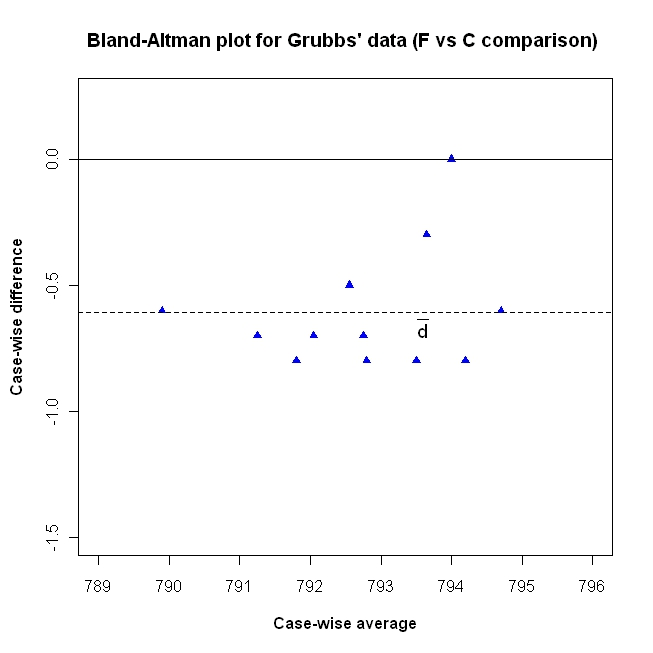
\includegraphics[width=120mm]{GrubbsBAplot-noLOA.jpeg}
		\caption{Bland-Altman plot For Fotobalk and Counter methods.}\label{GrubbsBA-noLOA}
	\end{center}
\end{figure}



In Figure 1.3 Bland-Altman plots for the `F vs C' and `F vs T'
comparisons are shown, where `F vs T' refers to the comparison of
the `Fotobalk' and `Terma' methods. Usage of the Bland-Altman plot
can be demonstrate in the contrast between these comparisons. By inspection, there exists a larger inter-method bias in the `F vs C' comparison than in the `F vs T' comparison. Conversely there
appears to be less precision in `F vs T' comparison, as indicated
by the greater dispersion of covariates.

\begin{figure}[h!]
	\begin{center}
		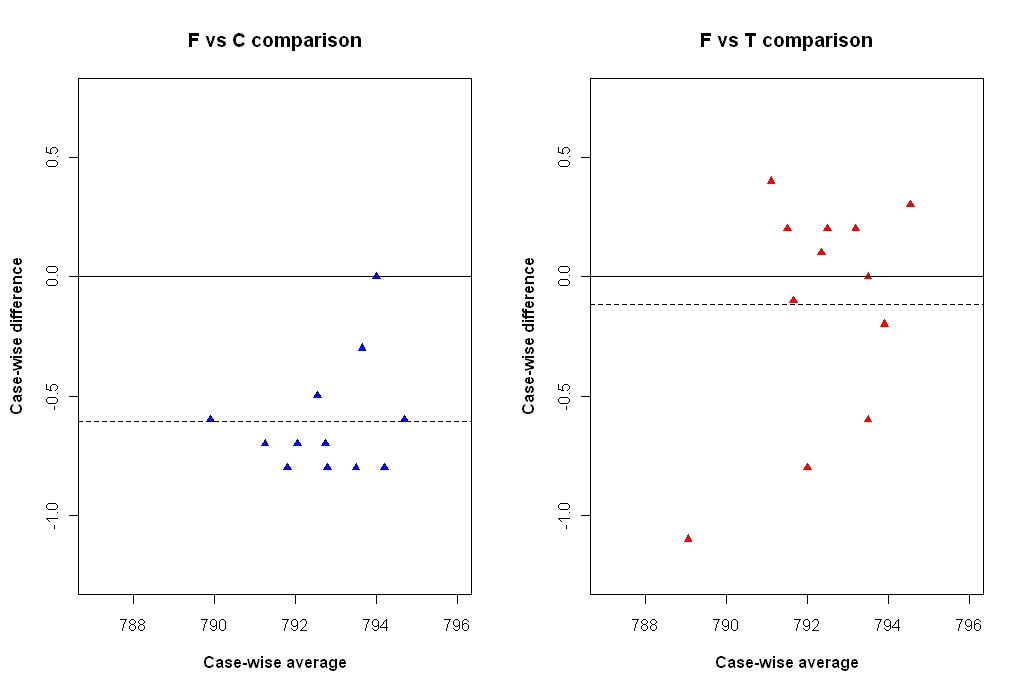
\includegraphics[height=90mm]{GrubbsDataTwoBAplots.jpeg}
		\caption{Bland-Altman plots for Grubbs' F vs C and F vs T comparisons.}\label{GrubbsDataTwoBAplots}
	\end{center}
\end{figure}

\newpage

\subsection{Prevalence of the Bland-Altman plot}
\citet*{BA86}, which further develops the Bland-Altman methodology,
was found to be the sixth most cited paper of all time by the
\citet{BAcite}. \cite{Dewitte} describes the rate at which prevalence of the Bland-Altman plot has developed in scientific
literature. \citet{Dewitte} reviewed the use of Bland-Altman plots by examining all articles in the journal `Clinical Chemistry' between 1995 and 2001. This study concluded that use of the Bland–Altman plot increased over the years, from 8\% in 1995 to 14\% in 1996, and 31–36\% in 2002.

The Bland-Altman Plot has since become expected, and
often obligatory, approach for presenting method comparison studies in many scientific journals \citep{hollis}. Furthermore \citet{BritHypSoc} recommend its use in papers pertaining to
method comparison studies for the journal of the British Hypertension Society.

\subsection{Adverse features}

Estimates for inter-method bias and variance of differences are only meaningful if there is uniform inter-bias and variability throughout the range of measurements. Fulfilment of these assumptions can be checked by visual inspection of the plot.The prototype Bland-Altman plots depicted in Figures 1.4, 1.5 and 1.6 are derived from simulated data, for the purpose of demonstrating how the plot would inform an analyst of features that would adversely affect use of the recommended methodology.

Figure 1.4 demonstrates how the Bland-Altman plot would indicate increasing variance of differences over the measurement range. Fitted regression lines, for both the upper and lower half of the plot, has been added to indicate the trend. Figure 1.5 is an example of cases where the inter-method bias changes over the measurement range. This is known as proportional bias, and is defined by \citet{ludbrook97} as meaning that `one method gives values that are higher (or lower) than those from the other by an amount that is proportional to the level of the measured variable'. In both Figures 1.4 and 1.5, the assumptions necessary for further analysis using the limits of agreement are violated.

Application of regression techniques to the Bland-Altman plot, and subsequent formal testing for the constant variability of
differences is informative. The data set may be divided into two subsets, containing the observations wherein the difference values
are less than and greater than the inter-method bias respectively.
For both of these fits, hypothesis tests for the respective slopes
can be performed. While both tests can be considered separately,
multiple comparison procedures, such as the Benjamini-Hochberg
\citep{BH} test, should be also be used.

\begin{figure}[h!]
	\begin{center}
		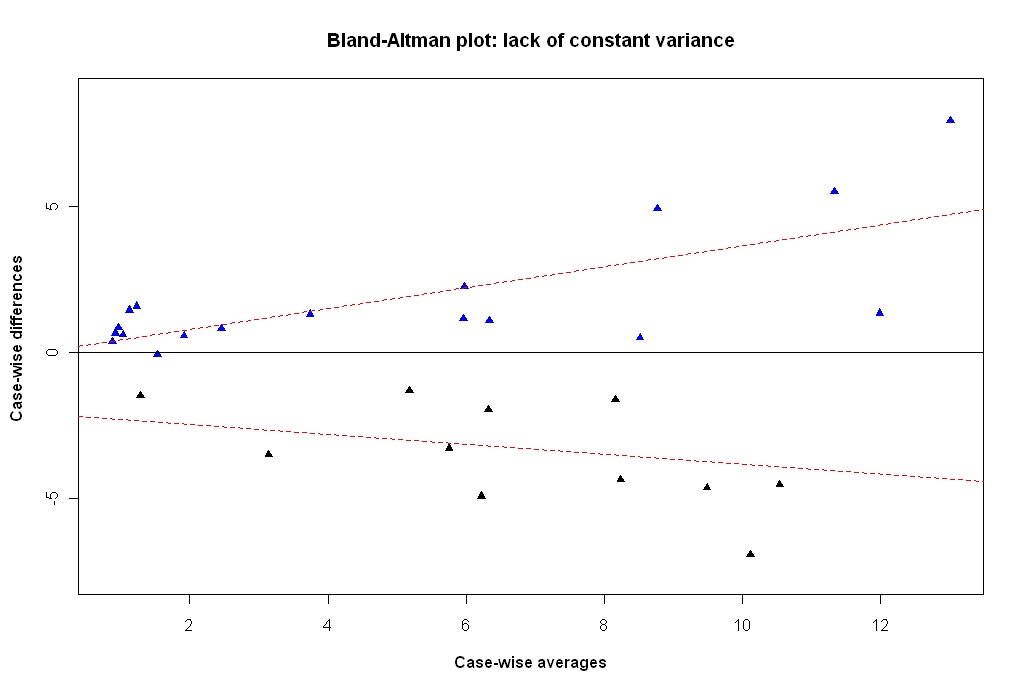
\includegraphics[height=90mm]{BAFanEffect.jpeg}
		\caption{Bland-Altman plot demonstrating the increase of variance over the range.}\label{BAFanEffect}
	\end{center}
\end{figure}

\begin{figure}[h!]
	\begin{center}
		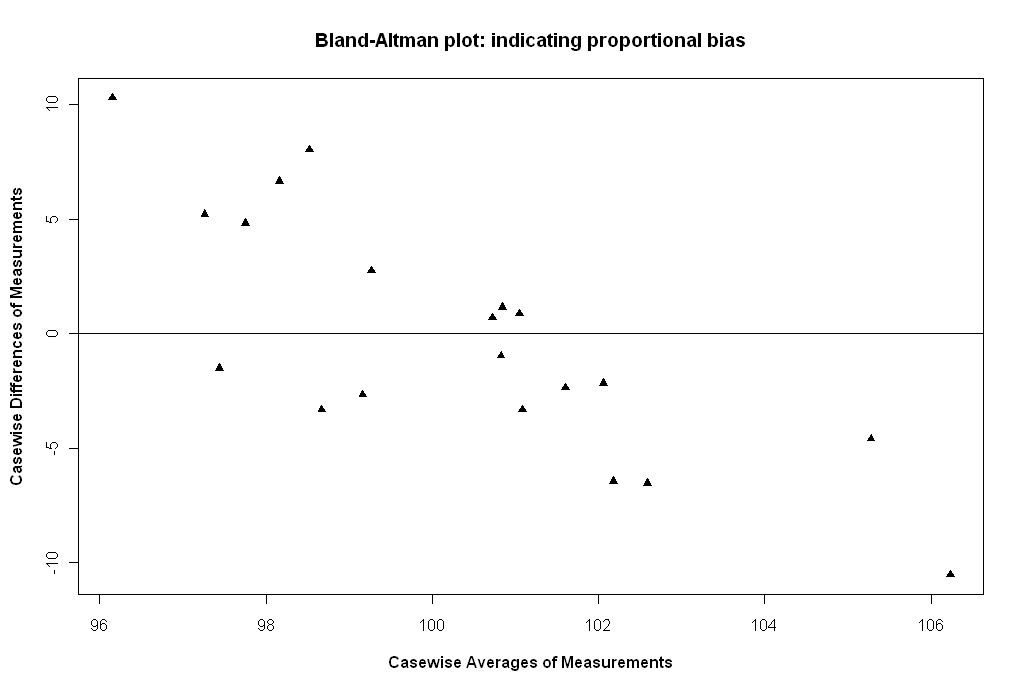
\includegraphics[height=90mm]{PropBias.jpeg}
		\caption{Bland-Altman plot indicating the presence of proportional bias.}\label{PropBias}
	\end{center}
\end{figure}

\begin{figure}[h!]
	\begin{center}
		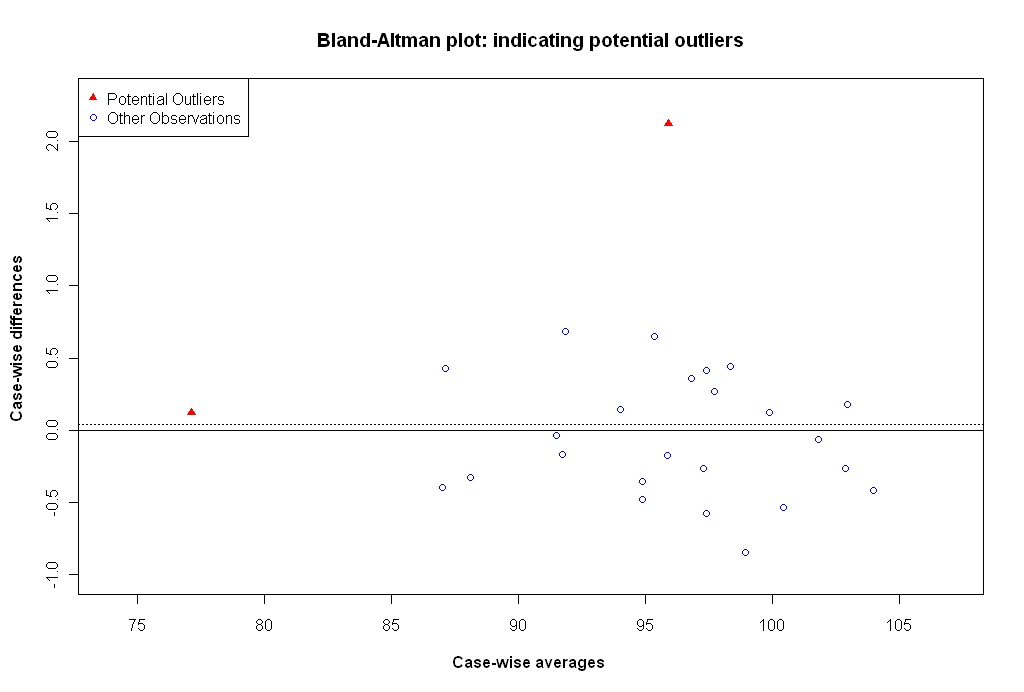
\includegraphics[width=125mm]{BAOutliers.jpeg}
		\caption{Bland-Altman plot indicating the presence of potential outliers.}\label{Outliers}
	\end{center}
\end{figure}

\newpage

% % OUTLIERS

The Bland-Altman plot also can be used to identify outliers. An outlier is an observation that is conspicuously different from the
rest of the data that it arouses suspicion that it occurs due to a mechanism, or conditions, different to that of the rest of the
observations. \citet*{BA99} do not recommend excluding outliers from analyzes, but remark that recalculation of the inter-method bias estimate,
and further calculations based upon that estimate, are useful for assessing the influence of outliers. The authors remark that `we
usually find that this method of analysis is not too sensitive to one or two large outlying differences'. Figure 1.6 demonstrates how the Bland-Altman
plot can be used to visually inspect the presence of potential outliers.

As a complement to the Bland-Altman plot, \citet{Bartko} proposes the use of a bivariate confidence ellipse, constructed for a
predetermined level. \citet{AltmanEllipse} provides the relevant calculations for the ellipse. This ellipse is intended as a visual guidelines for the scatter plot, for detecting outliers and to assess the within- and between-subject variances.

The minor axis relates to the between subject variability, whereas the major axis relates to the error mean square, with the ellipse
depicting the size of both relative to each other. Consequently Bartko's ellipse provides a visual aid to determining the
relationship between variances. If $\mbox{var}(a)$ is greater than $\mbox{var}(d)$, the orientation of the ellipse is horizontal. Conversely if $\mbox{var}(a)$ is less than $\mbox{var}(d)$, the orientation of the ellipse is vertical.


%(Furthermore \citet{Bartko}
%proposes formal testing procedures, that shall be discussed in due
%course.)

The Bland-Altman plot for the Grubbs data, complemented by Bartko's ellipse, is depicted in Figure 1.7. The fourth observation is shown to be outside the bounds of the ellipse, indicating that it is a potential outlier.


\begin{figure}[h!]
	% Requires \usepackage{graphicx}
	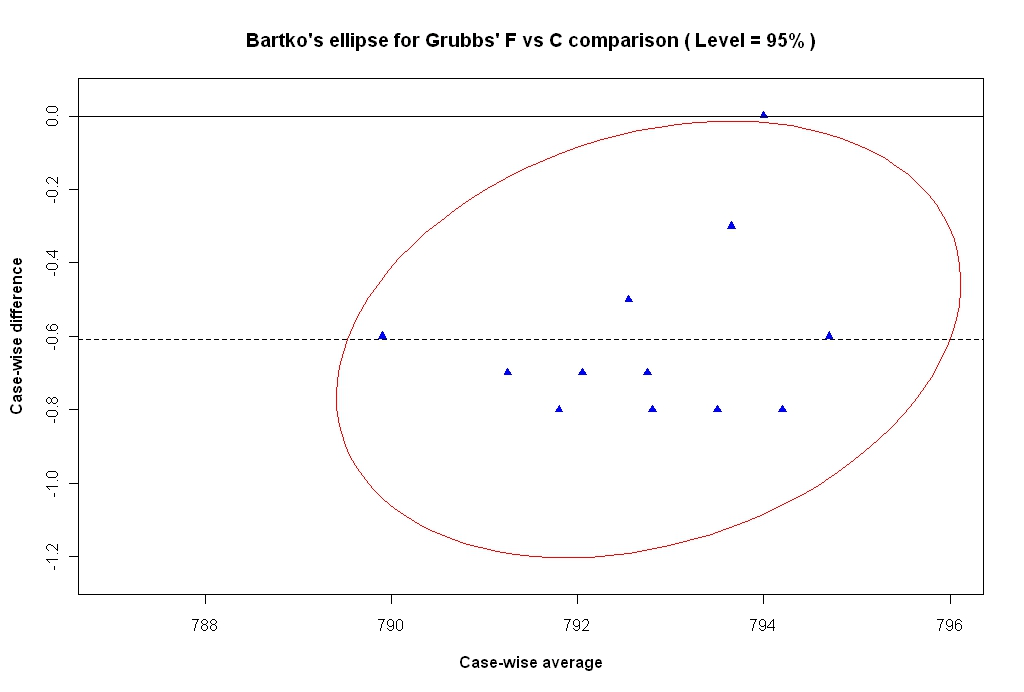
\includegraphics[width=130mm]{GrubbsBartko.jpeg}
	\caption{Bartko's Ellipse For Grubbs' Data.}\label{GrubbsBartko}
\end{figure}

The limitations of using bivariate approaches to outlier detection in the Bland-Altman plot can demonstrated using Bartko's ellipse.
A covariate is added to the `F vs C' comparison that has a difference value equal to the inter-method bias, and an average
value that markedly deviates from the rest of the average values in the comparison, i.e. 786. Table 1.8 depicts a $95\%$ confidence
ellipse for this manipulated data set. By inspection of the confidence interval, a conclusion would be reached that this extra
covariate is an outlier, in spite of the fact that this observation is wholly consistent with the conclusion of the
Bland-Altman plot.

\begin{figure}[h!]
	% Requires \usepackage{graphicx}
	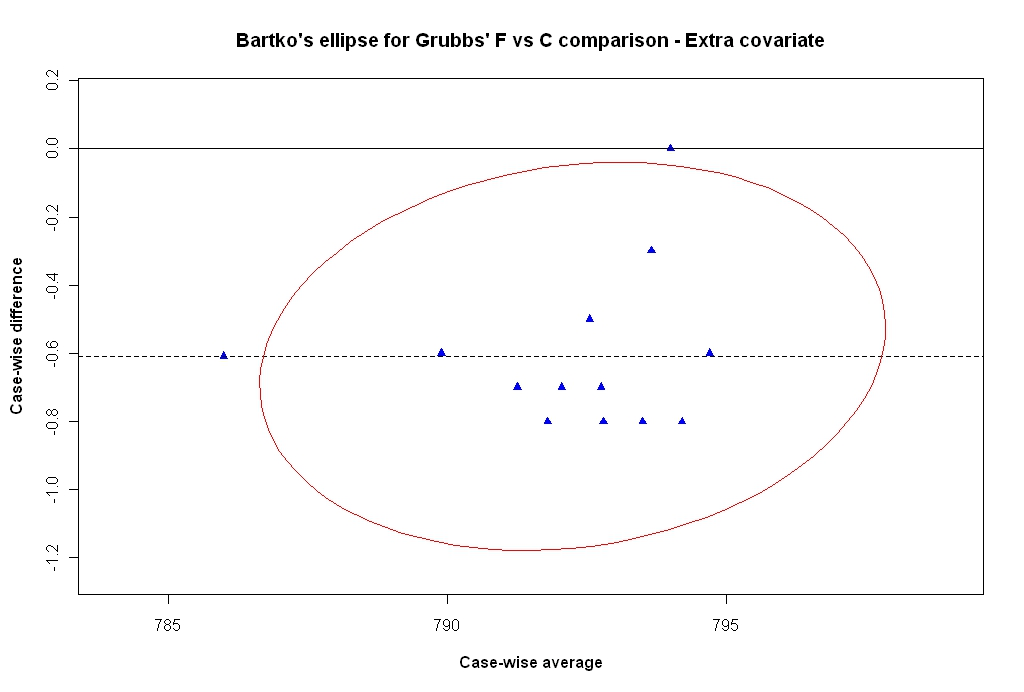
\includegraphics[width=130mm]{GrubbsBartko2.jpeg}
	\caption{Bartko's Ellipse For Grubbs' Data, with an extra covariate.}\label{GrubbsBartko2}
\end{figure}

Importantly, outlier classification must be informed by the logic of the data's formulation. In the Bland-Altman plot, the horizontal displacement of any
observation is supported by two independent measurements. Any observation should not be considered an outlier on the basis of a
noticeable horizontal displacement from the main cluster, as in the case with the extra covariate. Conversely, the fourth observation, from the original data set, should be considered an
outlier, as it has a noticeable vertical displacement from the rest of the observations.

%Grubbs' test is a statistical test used for detecting outliers in a
%univariate data set that is assumed to be normally distributed.

%\citet{Grubbs} defined an outlier as a co-variate that appears to
%deviate markedly from other members of the sample in which it
%occurs.

In classifying whether a observation from a univariate data set is an outlier, many formal tests are available, such as the Grubbs test for outliers. In assessing
whether a covariate in a Bland-Altman plot is an outlier, this test is useful when applied to the case-wise difference values treated as a
univariate data set. The null hypothesis of the Grubbs test procedure is the absence of any outliers in the data set. Conversely, the alternative hypotheses is that there is at least one outlier present.

The test statistic for the Grubbs test ($G$) is the largest absolute deviation from the sample mean divided by the standard deviation of the differences,
\[
G =  \displaystyle\max_{i=1,\ldots, n}\frac{\left \vert d_i -
	\bar{d}\right\vert}{S_{d}}.
\]

For the `F vs C' comparison it is the fourth observation gives rise to the test statistic, $G = 3.64$. The critical value is calculated using Student's $t$ distribution and the sample size,
\[
U = \frac{n-1}{\sqrt{n}} \sqrt{\frac{t_{\alpha/(2n),n-2}^2}{n - 2
		+ t_{\alpha/(2n),n-2}^2}}.
\]
For this test $U = 0.75$. The conclusion of this test is that the fourth observation in the `F vs C' comparison is an outlier, with $p-$value = 0.003, according with the previous result using Bartko's ellipse.

\newpage



\subsection{Inferences on Bland-Altman estimates}
\citet*{BA99}advises on how to calculate confidence intervals for the inter-method bias and limits of agreement. For the inter-method bias, the confidence interval is a simply that of a mean: $\bar{d} \pm t_{(0.5\alpha,n-1)} S_{d}/\sqrt{n}$.
The confidence intervals and standard error for the limits of agreement follow from the variance of the limits of agreement, which is shown to be

\[
\mbox{Var}(LoA) = (\frac{1}{n}+\frac{1.96^{2}}{2(n-1)})s_{d}^{2}.
\]

If $n$ is sufficiently large this can be following approximation
can be used
\[
\mbox{Var}(LoA) \approx 1.71^{2}\frac{s_{d}^{2}}{n}.
\]
Consequently the standard errors of both limits can be
approximated as $1.71$ times the standard error of the
differences.

A $95\%$ confidence interval can be determined, by means of the
\emph{t} distribution with $n-1$ degrees of freedom. However \citet*{BA99} comment that such calculations  may be `somewhat optimistic' on account of the associated assumptions not being realized.

%\subsubsection{Small Sample Sizes} The limits of agreement are
%estimates derived from the sample studied, and will differ from
%values relevant to the whole population, hence the importance of a
%suitably large sample size. A different sample would give
%different limits of agreement. Student's t-distribution is a well
%known probability distribution used in statistical inference for
%normally distributed populations when the sample size is small
%\citep{student,Fisher3}. Consequently, using 't' quantiles , as
%opposed to standard normal quantiles, may give a more appropriate
%calculation for limits of agreement when the sample size is small.
%For sample size $n=12$ the `t' quantile is 2.2 and the limits of
%agreement are (-0.074,-1.143).



\bibliography{DB-txfrbib}
\end{document}
